\documentclass[12pt]{article} 
\usepackage{amsmath} 
\usepackage{amsfonts}
\usepackage{amssymb} 
\usepackage[utf8]{inputenc} 
\usepackage[T1,T2A]{fontenc}
\usepackage[english, russian]{babel} 
\usepackage{graphicx}
\usepackage{float}
\usepackage[left=2cm,right=2cm,top=2cm,bottom=2cm]{geometry}
\usepackage{wrapfig}
\usepackage{pgfplots} 
\usepackage{setspace} 
\usepackage{indentfirst}
\usepackage{subfigure} 
\usepackage{hyperref}
\usepackage{mathrsfs}

\hypersetup{
    colorlinks=true,
    linkcolor=red,
    urlcolor=magenta,
}

\graphicspath{{pictures}}

\title{ 
    Лабораторная работа 2.4.1 \\
    <<Определение теплоты испарения жидкости>>
}

\author{Балдин Виктор, Б01-303}

\begin{document}
    \maketitle
    \paragraph{Цель работы}
    \begin{enumerate}
        \item Измерение давления насыщенного пара жидкости при различной 
        температуре.
        \item Вычисление теплоты испарения с помощью уравнения Клайперона-
        Клаузиуса.
    \end{enumerate}
    \paragraph{Оборудование} Термостат, герметичный сосуд, заполненный
    исследумеой жидкостью, отсчетный микроскоп.
    
    \section{Теоретическая часть}
    Для теплоты испарения можно записать уравнение Клайперона-Клаузиуса:
    \begin{equation}
        \frac{dP}{dT} = \frac{L}{T(V_2 - V_1)},
        \label{klaus}
    \end{equation}
    где $V_2$ -- объем газа, $V_1$ -- объем жидкости.
    
    В данном случае мы используем модель идеального газа применительно
    к парам исследуемой жидкости:
    \begin{equation}
        V = \frac{RT}{P}
        \label{klaip}
    \end{equation}
    
    Объединяя \ref{klaus} и \ref{klaip}, получим:
    \begin{equation}
        L = \frac{RT^2}{P}\frac{dP}{dT} = -R\frac{d(\ln P)}{d(1 / T)}
    \end{equation}
    
    \section{Установка}
    Схема экспериментальной установки приведена на рисунке \ref{stand}.
    
    \begin{figure}[h!]
        \centering
        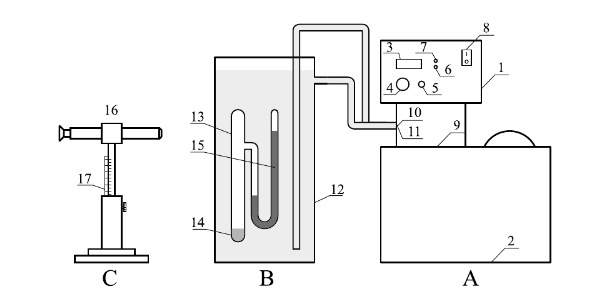
\includegraphics[scale=1]{stand.png}
        \caption{Схема установки для определения удельной теплоты испарения}
        \label{stand}
    \end{figure}
    
    \section{Ход работы}
    \begin{enumerate} 
        \item Измерим разность уровней в ртутном U-образом манометре с помощью
        микроскопа.
        \item Включим термостат.
        \item Будем измерять давление насыщенного пара с интервалом 1 \textdegree C.
        \begin{figure}[h!]
            \centering
            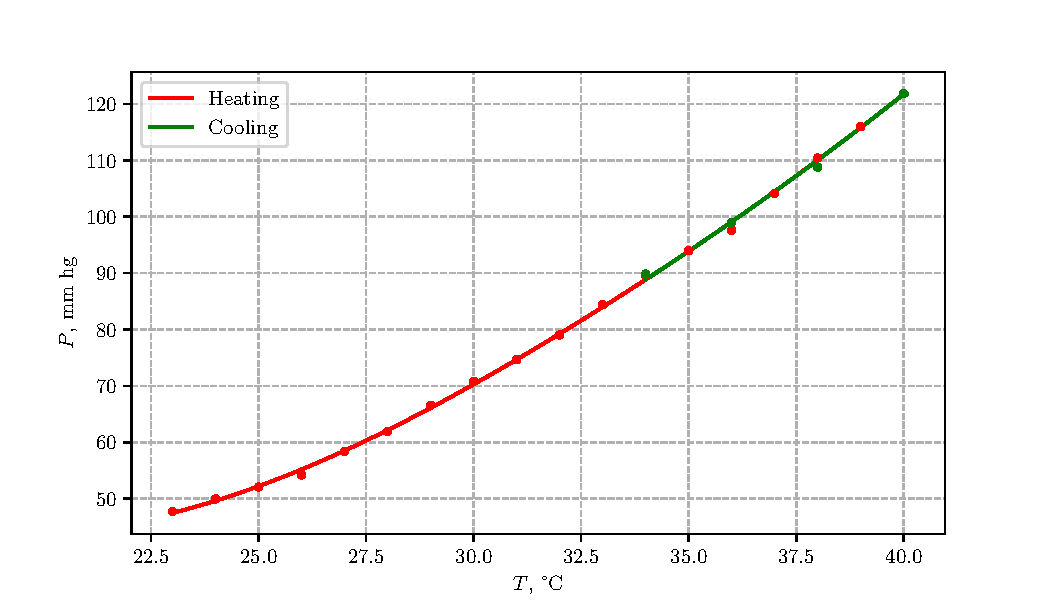
\includegraphics{data/curve.pdf}
            \caption{Зависимость $P(T)$}
        \end{figure}
        
        \begin{figure}[h!]
            \centering
            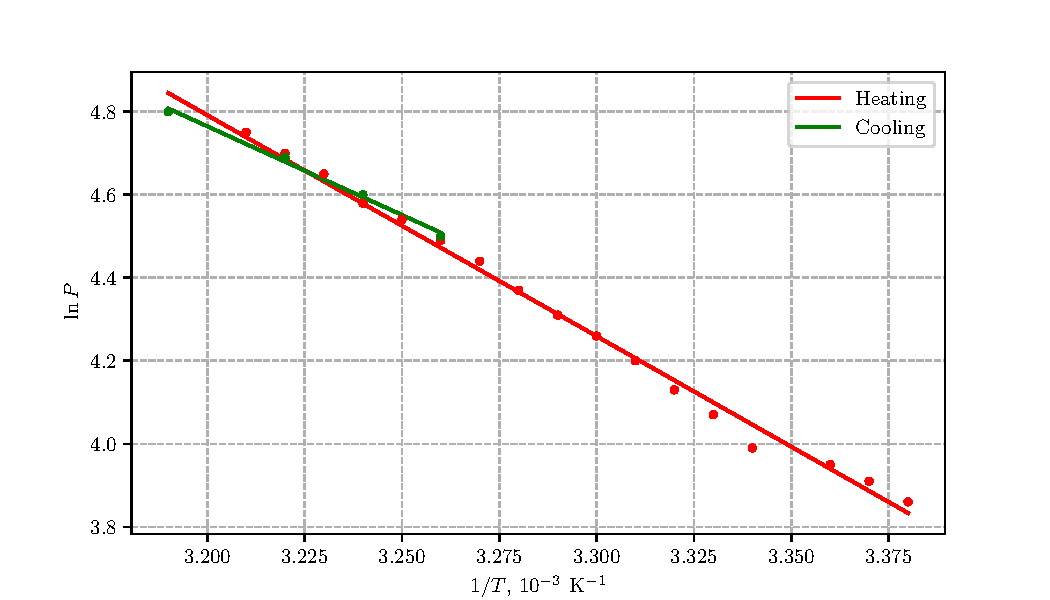
\includegraphics{data/lin.pdf}
            \caption{Линеаризованная зависимость $\ln P(1 / T)$}
        \end{figure}    
    \end{enumerate}
    
\end{document}
